\documentclass{standalone}
\usepackage{tikz}

\begin{document}

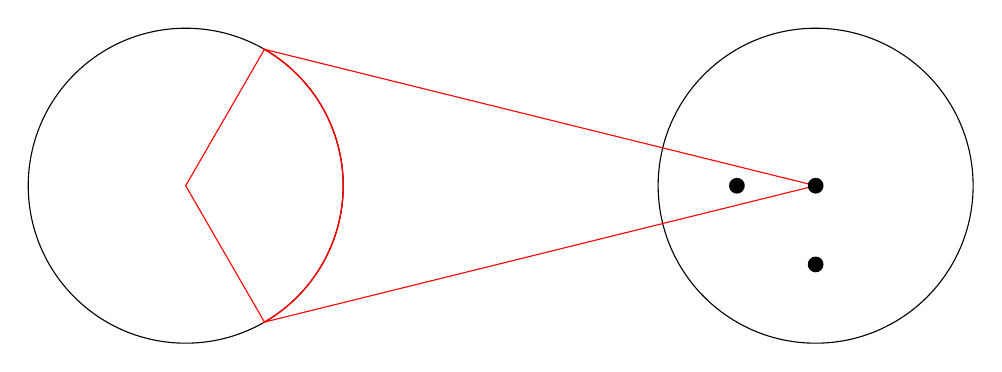
\begin{tikzpicture}[scale=2]
    % Circle 1
    \draw (0,0) circle (1);
    \draw[red] (0,0) -- (60:1) arc (60:-60:1) -- cycle;
    
    % Circle 2
    \draw (4,0) circle (1);
    \draw[red] (4,0) -- (60:1) arc (60:-60:1) -- cycle;
    \fill (4,0) circle (0.05); % Black dot
    
    % Circle 2 - second black dot
    \fill (4,0) ++(180:0.5) circle (0.05); % Black dot at 180 degrees
    
    % Circle 2 - third black dot
    \fill (4,0) ++(-90:0.5) circle (0.05); % Black dot at -90 degrees
\end{tikzpicture}

\end{document}